\documentclass[conference]{IEEEtran}
\IEEEoverridecommandlockouts
% The preceding line is only needed to identify funding in the first footnote. If that is unneeded, please comment it out.
\usepackage{cite}
\usepackage{amsmath,amssymb,amsfonts}
\usepackage{algorithmic}
\usepackage{graphicx}
\usepackage{textcomp}
\usepackage{xcolor}
\usepackage[brazilian]{babel}
\usepackage[utf8]{inputenc}
\usepackage[T1]{fontenc}
\usepackage{listings}
\usepackage{color}
\usepackage{float}
\usepackage{multirow}
\usepackage{hyperref}

\definecolor{dkgreen}{rgb}{0,0.6,0}
\definecolor{gray}{rgb}{0.5,0.5,0.5}
\definecolor{mauve}{rgb}{0.58,0,0.82}

\lstset{frame=tb,
  language=Java,
  aboveskip=3mm,
  belowskip=3mm,
  showstringspaces=false,
  columns=flexible,
  basicstyle={\small\ttfamily},
  numbers=none,
  numberstyle=\tiny\color{gray},
  keywordstyle=\color{blue},
  commentstyle=\color{dkgreen},
  stringstyle=\color{mauve},
  breaklines=true,
  breakatwhitespace=true,
  tabsize=3
}
\lstset{language=Python}
\def\BibTeX{{\rm B\kern-.05em{\sc i\kern-.025em b}\kern-.08em
    T\kern-.1667em\lower.7ex\hbox{E}\kern-.125emX}}
\begin{document}

\title{Relatório do Laboratório 8: \\ Imitation Learning com Keras\\
}

\author{\IEEEauthorblockN{Isabelle Ferreira de Oliveira}
\IEEEauthorblockA{\textit{CT-213 - Engenharia da Computação 2020} \\
\textit{Instituto Tecnológico de Aeronáutica (ITA)}\\
São José dos Campos, Brasil \\
isabelle.ferreira3000@gmail.com}
}

\maketitle

\begin{abstract}
Esse relatório documenta a cópia de um movimento de caminhada de um robô humanoide usando a técnica chamada \textit{imitation learning}. Para isso, foi utilizado o \textit{framework} de \textit{Deep Learning} Keras, que facilita o uso do \textit{framework} Tensorflow.
\end{abstract}

\begin{IEEEkeywords}
\textit{Imitation learning}, \textit{deep learning}, Keras, Tensorflow
\end{IEEEkeywords}

\section{Introdução}
\textit{Deep learning} é um tipo de aprendizado de máquina que treina para aprender através do reconhecimento de padrões em várias camadas de processamento. Entre as tarefas possíveis realizáveis estão o reconhecimento de fala, identificação de imagem e previsões, entre outras tarefas realizadas por seres humanos. 

Esse tipo de estratégia possibilita, também, aprender por imitação. Assim, o comportamento desejado (uma política de controle, por exemplo) é copiado usando aprendizado supervisionado.

O \textit{framework} Keras facilita o uso do \textit{framework} Tensorflow para problemas de \textit{Deep learning}, transformando a implementação, treino e resultado da rede neural em chamadas de API. O funcionamento dessas chamadas pode ser visto a seguir. Em seguida, será apresentado como isso foi aplicado no contexto do laboratório.

\begin{lstlisting}
from keras import models

# Creates the neural network model in Keras
model = models.Sequential()
\end{lstlisting}

\textit{Sequential()} cria uma pilha linear de camadas.

\begin{lstlisting}
from keras import layers, activations, regularizers

# Adds the first layer
model.add(layers.Dense(num_neurons,
	activation=activations.some_function,
	input_shape=(input_size,),
	kernel_regularizer=regularizers.l2(lambda)))

# Adds another layer (not first)
model.add(layers.Dense(num_neurons,
	activation=activations.some_function,
	kernel_regularizer=regularizers.l2(lambda)))
\end{lstlisting}

Para a criação de uma camada na rede neural através do Keras, utiliza-se a função \textit{model.add(layers.Dense())}, sendo o primeiro argumento referente ao número de neurônios nessa camada; "activation" configura a função de ativação; "input\underline{\space}shape" representa o tamanho da entrada; e "kernel\underline{\space}regularizer" configura a regularização para essa camada.

\begin{lstlisting}
from keras import losses, optimizers, metrics

# Configures the model for training
model.compile(optimizer=optimizers.Adam(),
	loss=losses.binary_crossentropy,
	metrics=[metrics.binary_accuracy])

# Trains the model for a given number of epochs
history = model.fit(inputs,
	expected_outputs,
	batch_size=size_of_batch,
	epochs=num_epochs)

\end{lstlisting}

Por fim, configura-se o modelo para o treino, escolhendo o otimizer, a função de custo e as métricas; e se treina o modelo para um determinado conjunto de entrada, tendo as saídas esperadas, o tamanho do batch e quantas épocas serão efetuadas.

\section{Implementação}
Para a implementação da rede neural conforme os parâmetros requisitados pelo roteiro do laboratório \cite{roteiro} e apresentada na tabela da Figura \ref{arquitetura_rede_neural}, era necessário utilizar do código de adição de camadas a uma rede, além de configuração e treino do modelo, apresentado na Introdução. 

Tendo em vista que em \textit{keras.activations} não há função de ativação Leaky ReLU, utilizou-se a recomendação sugerida pelo roteiro \cite{roteiro} para usar Leaky ReLU no Keras, ou seja, foi adicionado uma camada do tipo LeakyRelu após ter definido uma camada (usando função de ativação linear).

Além disso, para configurar o modelo, setou-se o parâmetro \textit{loss} da função \textit{compile()} para \textit{losses.mean\underline{\space}squared\underline{\space}error}, uma vez que foi utilizado erro quadrático.

Por fim, para treinar, o tamanho do \textit{batch} foi o tamanho total de entradas, para que seja usado todo o \textit{dataset} em cada iteração do treinamento.

\begin{figure}[htbp]
\centering
\centerline{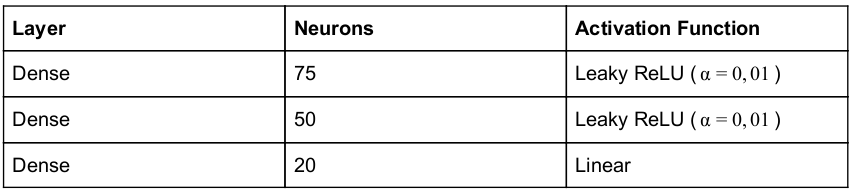
\includegraphics[scale=0.3]{imagens/arquitetura_rede_neural.png}}
\caption{Arquitetura da rede neural usada para o imitation learning. Essa imagem foi apresentada no roteiro \cite{roteiro}}.
\label{arquitetura_rede_neural}
\end{figure}

\section{Resultados e Conclusões}

\subsection{Estudo de implementação de Rede Neural com Keras}
O código do arquivo \textit{test\underline{\space}keras.py} foi estudado para se entender a utilização do \textit{framework} Keras na implementação de redes neurais. O que foi aprendido resultou no texto escrito na Introdução.

\subsection{Análise do efeito de Regularização}
Esse arquivo \textit{test\underline{\space}keras.py} continha a implentação do aprendizado das funções "soma maior que zero" e "xor" para diferentes valores de regularização.

Após a execução desse arquivo, obteve-se os resultados apresentados nas Figuras de \ref{sum_gt_zero/lambda_zero/dataset_sgz} a \ref{xor/nn_classification_xor}, sendo as Figuras \ref{sum_gt_zero/lambda_zero/dataset_sgz} e \ref{xor/lambda_zero/dataset_xor} os \textit{dataset} utilizados para as funções "soma maior que zero" e "xor", respectivamente.

Analisando os resultados, é possível notar que em todas as situações (com e sem regularização, e para as duas funções) a rede obtive uma classificação satisfatória. A classificação com regularização, entretando, apresentou-se muito mais acertiva, conforme se pode observar pelas comparação das Figuras \ref{sum_gt_zero/lambda_zero/nn_classification_sgz} e \ref{sum_gt_zero/nn_classification_sgz} para "soma maior que zero" e \ref{xor/lambda_zero/nn_classification_xor} e \ref{xor/nn_classification_xor} para "xor". 

A questão da convergência da função de custo também pode ser comparada. Para os casos com regularização, a convergência se deu bem antes em número de épocas. Isso pode ser observado nas Figuras \ref{sum_gt_zero/lambda_zero/convergence_sgz} e \ref{sum_gt_zero/convergence_sgz}, para "soma maior que zero" e nas Figuras \ref{xor/lambda_zero/convergence_xor} e \ref{xor/convergence_xor} para "xor". 

\begin{figure}[htbp]
\centering
\centerline{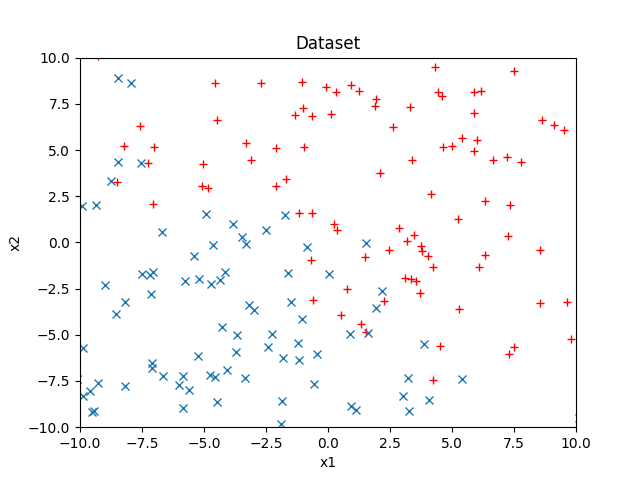
\includegraphics[scale=0.5]{imagens/sum_gt_zero/lambda_zero/dataset_sgz.png}}
\caption{\textit{Dataset} utilizado para o aprendizado da função $soma > 0$}.
\label{sum_gt_zero/lambda_zero/dataset_sgz}
\end{figure}

\begin{figure}[htbp]
\centering
\centerline{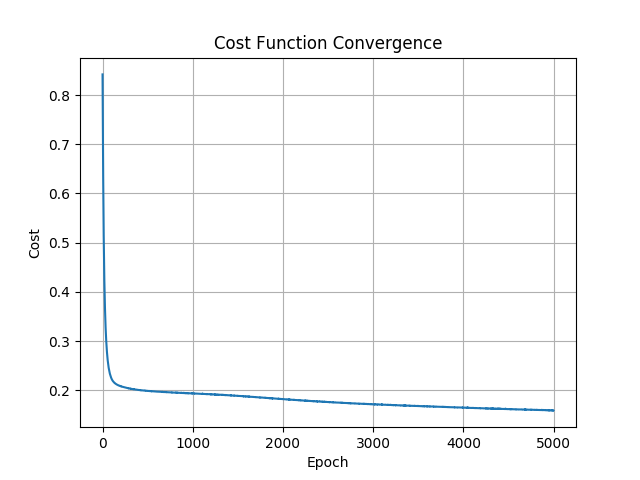
\includegraphics[scale=0.5]{imagens/sum_gt_zero/lambda_zero/convergence_sgz.png}}
\caption{Convergência da função de custo para a função $soma > 0$, sem regularização.}.
\label{sum_gt_zero/lambda_zero/convergence_sgz}
\end{figure}

\begin{figure}[htbp]
\centering
\centerline{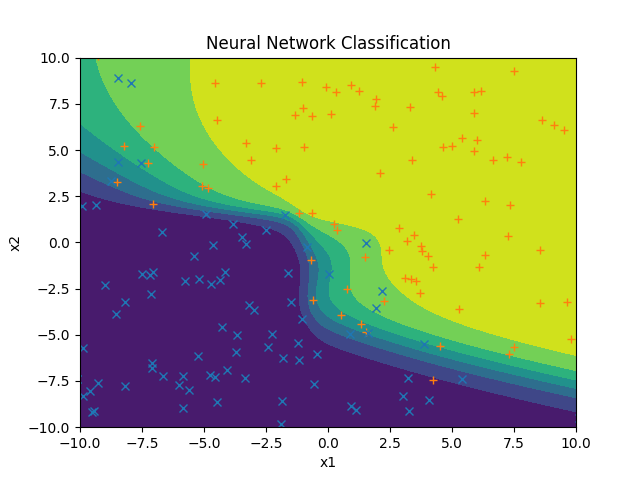
\includegraphics[scale=0.5]{imagens/sum_gt_zero/lambda_zero/nn_classification_sgz.png}}
\caption{Resultado da classificação por rede neural para a função $soma > 0$, sem regularização.}
\label{sum_gt_zero/lambda_zero/nn_classification_sgz}
\end{figure}

\begin{figure}[htbp]
\centering
\centerline{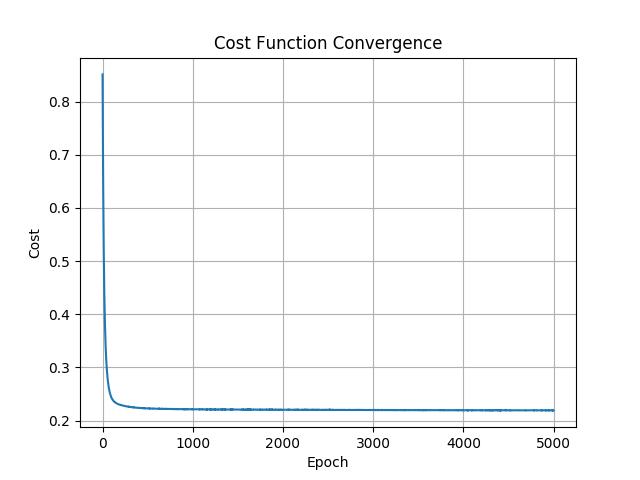
\includegraphics[scale=0.5]{imagens/sum_gt_zero/convergence_sgz.png}}
\caption{Convergência da função de custo para a função $soma > 0$, com regularização.}
\label{sum_gt_zero/convergence_sgz}
\end{figure}

\begin{figure}[htbp]
\centering
\centerline{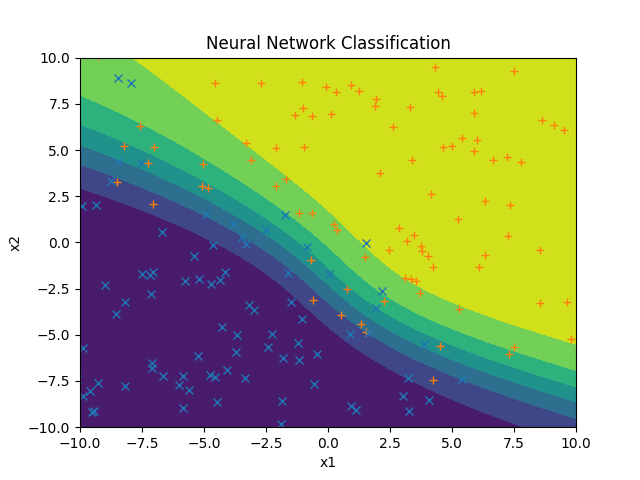
\includegraphics[scale=0.5]{imagens/sum_gt_zero/nn_classification_sgz.png}}
\caption{Resultado da classificação por rede neural para a função $soma > 0$, com regularização.}
\label{sum_gt_zero/nn_classification_sgz}
\end{figure}

\begin{figure}[htbp]
\centering
\centerline{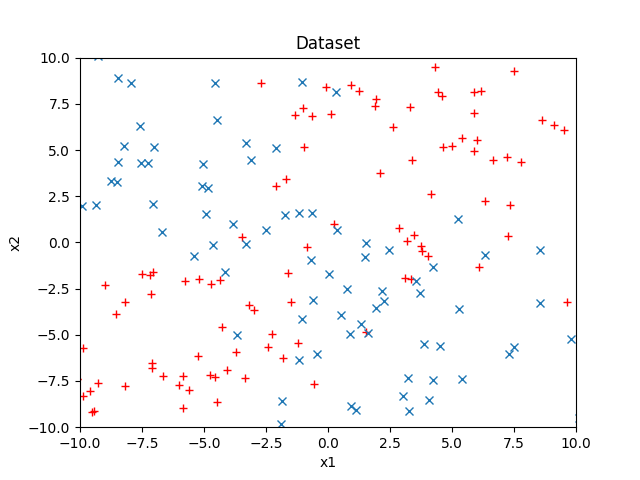
\includegraphics[scale=0.5]{imagens/xor/lambda_zero/dataset_xor.png}}
\caption{\textit{Dataset} utilizado para o aprendizado da função $xor$.}
\label{xor/lambda_zero/dataset_xor}
\end{figure} 

\begin{figure}[htbp]
\centering
\centerline{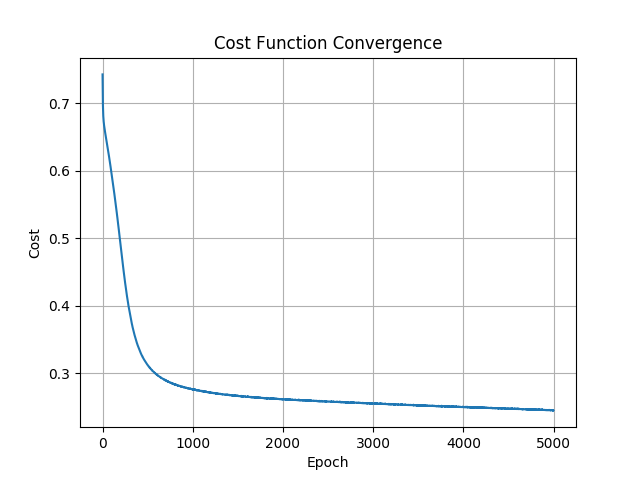
\includegraphics[scale=0.5]{imagens/xor/lambda_zero/convergence_xor.png}}
\caption{Convergência da função de custo para a função $xor$, sem regularização.}
\label{xor/lambda_zero/convergence_xor}
\end{figure}

\begin{figure}[htbp]
\centering
\centerline{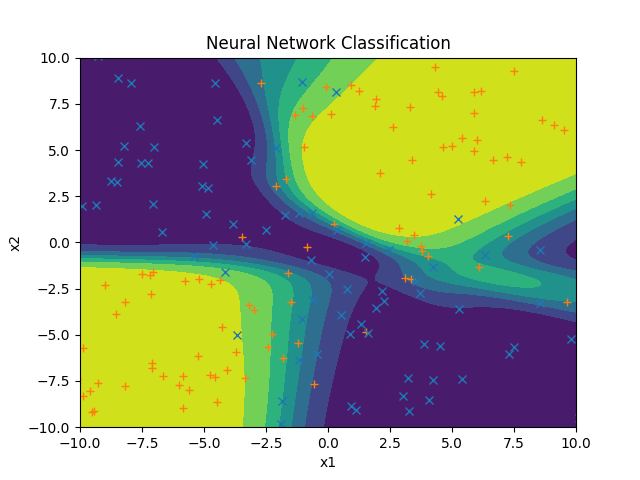
\includegraphics[scale=0.5]{imagens/xor/lambda_zero/nn_classification_xor.png}}
\caption{Resultado da classificação por rede neural para a função $xor$, sem regularização.}
\label{xor/lambda_zero/nn_classification_xor}
\end{figure}

\begin{figure}[htbp]
\centering
\centerline{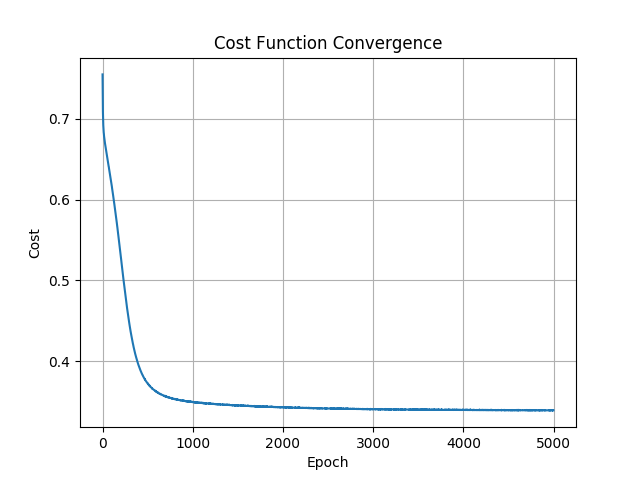
\includegraphics[scale=0.5]{imagens/xor/convergence_xor.png}}
\caption{Convergência da função de custo para a função $xor$, com regularização.}
\label{xor/convergence_xor}
\end{figure}

\begin{figure}[htbp]
\centering
\centerline{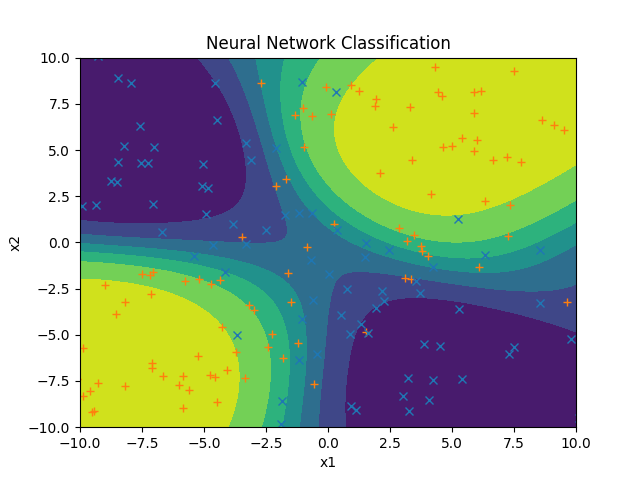
\includegraphics[scale=0.5]{imagens/xor/nn_classification_xor.png}}
\caption{Resultado da classificação por rede neural para a função $xor$, com regularização.}
\label{xor/nn_classification_xor}
\end{figure}

\subsection{Imitation Learning}
Após a implementação da rede neural com Keras conforme o explicado na seção Implementação, os resultados obtidos estão apresentados nas Figuras de \ref{imitation_learning/rightAnklePitch} a \ref{imitation_learning/rightKneePitch}. A comparação entre os gráficos de azul (curva original) e laranja (função aprendida por rede neural) dessas figuras demonstra que a implementação aconteceu de maneira satisfatória, uma vez que as funções ficaram bastante semelhantes.

\begin{figure}[htbp]
\centering
\centerline{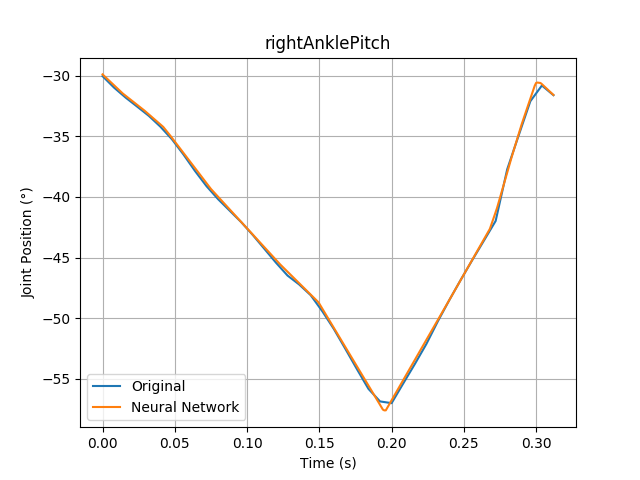
\includegraphics[scale=0.5]{imagens/imitation_learning/rightAnklePitch.png}}
\caption{Resultado da classificação por rede neural para a função \textit{soma > 0}.}
\label{imitation_learning/rightAnklePitch}
\end{figure} 

\begin{figure}[htbp]
\centering
\centerline{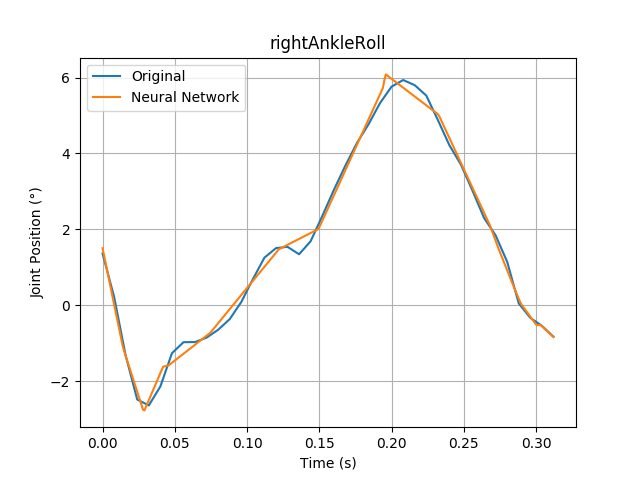
\includegraphics[scale=0.5]{imagens/imitation_learning/rightAnkleRoll.png}}
\caption{Resultado do \textit{Imitation learning} para Right Ankle Roll.}
\label{imitation_learning/rightAnkleRoll}
\end{figure}

\begin{figure}[htbp]
\centering
\centerline{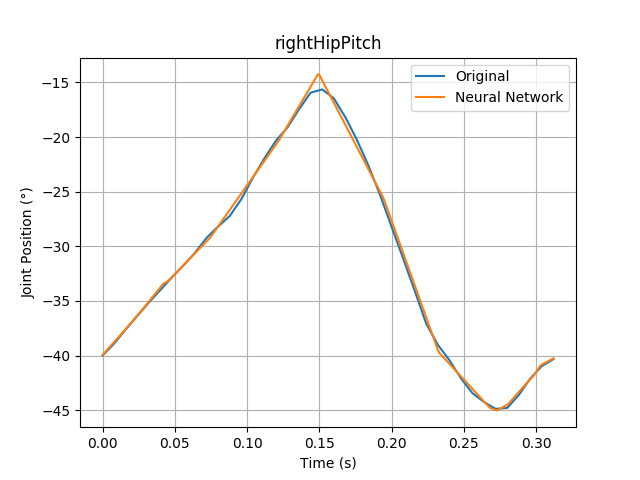
\includegraphics[scale=0.5]{imagens/imitation_learning/rightHipPitch.png}}
\caption{Resultado do \textit{Imitation learning} para Right Hip Pitch.}
\label{imitation_learning/rightHipPitch}
\end{figure}

\begin{figure}[htbp]
\centering
\centerline{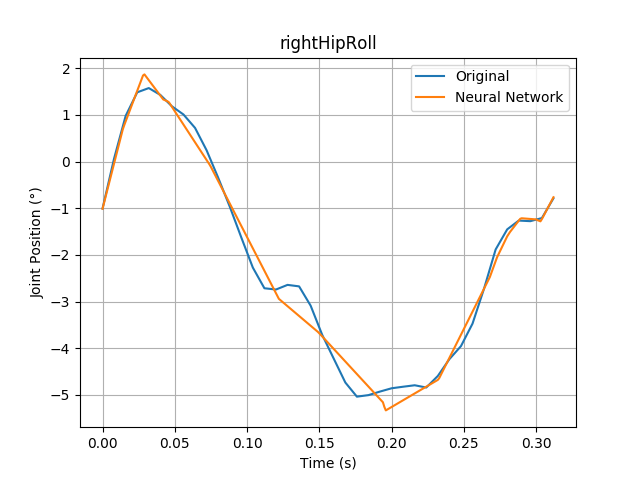
\includegraphics[scale=0.5]{imagens/imitation_learning/rightHipRoll.png}}
\caption{Resultado do \textit{Imitation learning} para Right Hip Roll.}
\label{imitation_learning/rightHipRoll}
\end{figure}

\begin{figure}[htbp]
\centering
\centerline{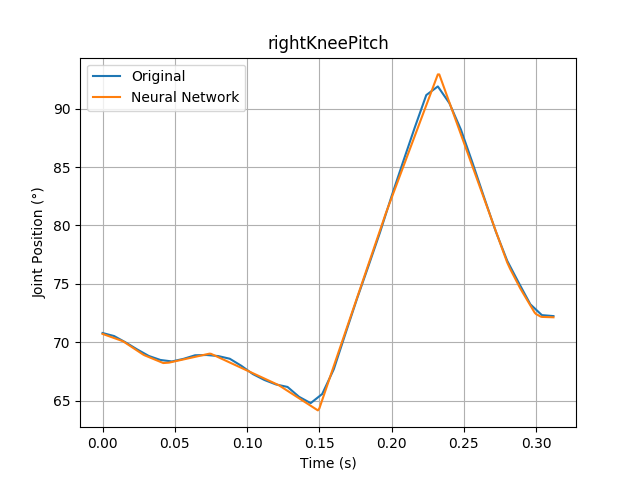
\includegraphics[scale=0.5]{imagens/imitation_learning/rightKneePitch.png}}
\caption{Resultado do \textit{Imitation learning} para Right Knee Pitch.}
\label{imitation_learning/rightKneePitch}
\end{figure}

Tendo em vista o que foi apresentado, pode-se notar, por fim, que algoritmos de \textit{Deep leaning} e o \textit{framework} Keras realmente se demonstraram eficazes em realizar aprendizado por imitação.

\begin{thebibliography}{00}
\bibitem{roteiro} M. Maximo, ``Roteiro: Laboratório 8 - Imitation Learning com Keras''. Instituto Tecnológico de Aeronáutica, Departamento de Computação. CT-213, 2019.
\end{thebibliography}

\end{document}
